\documentclass[journal]{IEEEtran}
\usepackage{amsmath,booktabs,graphicx,microtype,array}
\usepackage[hidelinks]{hyperref}
\makeatletter
\setlength{\@fptop}{0pt}\setlength{\@fpsep}{5pt}\setlength{\@fpbot}{0pt plus 1fil}
\setlength{\@dblfptop}{0pt}\setlength{\@dblfpsep}{5pt}\setlength{\@dblfpbot}{0pt plus 1fil}
\makeatother
\emergencystretch=2em\sloppy
\title{Supplementary Material for ``Coverage-Qualified Evaluation-Contract Auditing for Aerial Vehicle Detection''}
\author{Xinling Wen, Jiahao Zhang, Wenqi Liu, Yangxu Ren, and Yu Chen}
\begin{document}\maketitle
\renewcommand{\thesection}{S\arabic{section}}
\renewcommand{\thetable}{S\arabic{table}}
\setcounter{page}{1}

\section{Registered Contracts and Count Ledger}
The four contracts alter one evaluator factor at a time. All detections are score ordered; retained valid GT is matched before an otherwise unmatched detection can be neutralized. Removed and source-ignore regions use intersection over prediction area at .5. Table~\ref{tab:contracts} distinguishes the scored target from neutral regions explicitly.

\begin{table}[!t]
\centering
\caption{Registered evaluation contracts. $G$ is all valid GT, $G_t$ the support-retained target, $D_t=G\setminus G_t$, and $H$ source ignore.}\label{tab:contracts}
\scriptsize
\setlength{\tabcolsep}{1.8pt}\renewcommand{\arraystretch}{1.05}
\begin{tabular}{clll}
\toprule
ID & Scored valid GT & Neutral regions & Step meaning\\
\midrule
$A$ & $G$ & none & all-valid reference\\
$F$ & $G_t$ & none & removed objects are background\\
$R$ & $G_t$ & $D_t$ & neutralize removed objects\\
$S$ & $G_t$ & $D_t\cup H$ & add source ignores\\
\bottomrule
\end{tabular}
\end{table}

Table~\ref{tab:ledger} is the support-conditioned count-transition ledger behind Fig.~2 of the main paper. Every row is an exact adjacent-contract difference for one fixed prediction artifact. Summing the three $\Delta F_1$ values gives $F_{1,S}-F_{1,A}$ to machine precision. Because $F_1$ is nonlinear, the values are path-specific transitions rather than additive causal effects that are invariant to reordering.

\begin{table}[!t]
\centering
\caption{Exact TP/FP/FN transition ledger at confidence and IoU .25. A = absolute 24 px; N = normalized .015. AI-TOD is conditioned on its 1,869 covered images.}\label{tab:ledger}
\tiny
\setlength{\tabcolsep}{1.0pt}\renewcommand{\arraystretch}{.96}
\begin{tabular}{llcrrrrr}
\toprule
Source & Rule & Step & $\Delta$TP & $\Delta$FP & $\Delta$FN & $\Delta$neutral & $\Delta F_1$\\
\midrule
VisDrone & A & $A\to F$ & $-2256$ & $+2256$ & $-2288$ & 0 & $-.0360$\\
         &   & $F\to R$ & 0 & $-2320$ & 0 & $+2320$ & $+.0667$\\
         &   & $R\to S$ & 0 & $-293$  & 0 & $+293$  & $+.0093$\\
VisDrone & N & $A\to F$ & $-399$ & $+399$ & $-1344$ & 0 & $+.0178$\\
         &   & $F\to R$ & 0 & $-356$ & 0 & $+356$ & $+.0093$\\
         &   & $R\to S$ & 0 & $-294$ & 0 & $+294$ & $+.0078$\\
\midrule
UAVDT & A & $A\to F$ & $-301$ & $+301$ & $-237$ & 0 & $-.0085$\\
      &   & $F\to R$ & 0 & $-547$ & 0 & $+547$ & $+.0038$\\
      &   & $R\to S$ & 0 & 0 & 0 & 0 & $.0000$\\
UAVDT & N & $A\to F$ & $-105$ & $+105$ & $-182$ & 0 & $-.0023$\\
      &   & $F\to R$ & 0 & $-193$ & 0 & $+193$ & $+.0014$\\
      &   & $R\to S$ & 0 & 0 & 0 & 0 & $.0000$\\
\midrule
AI-TOD & A & $A\to F$ & $-11977$ & $+11977$ & $-2890$ & 0 & $-.3303$\\
       &   & $F\to R$ & 0 & $-30232$ & 0 & $+30232$ & $+.0800$\\
       &   & $R\to S$ & 0 & 0 & 0 & 0 & $.0000$\\
AI-TOD & N & $A\to F$ & $-5707$ & $+5707$ & $-1840$ & 0 & $-.1359$\\
       &   & $F\to R$ & 0 & $-12587$ & 0 & $+12587$ & $+.0660$\\
       &   & $R\to S$ & 0 & 0 & 0 & 0 & $.0000$\\
\bottomrule
\end{tabular}
\end{table}

\section{Coverage Qualification and Full Support Grid}
Raw prediction names establish coverage before class filtering. VisDrone and UAVDT cover all declared images. AI-TOD covers 1,869/2,804 images and is therefore eligible for full-annotation support diagnosis, a covered-subset metric replay, but not full-benchmark metric or rank inference. Its 1,869 covered images contain 16,900 boxes; the 935 noncovered images contain 43,004.

\begin{table}[!t]
\centering
\caption{AI-TOD covered--noncovered image qualification. Brackets are median [Q1,Q3]. SMD uses covered minus noncovered means; $W_1$ is in the feature's native unit.}\label{tab:coverage}
\tiny
\setlength{\tabcolsep}{1.5pt}\renewcommand{\arraystretch}{1.04}
\begin{tabular}{lrrrr}
\toprule
Feature & Covered & Noncovered & SMD & $W_1$\\
\midrule
Boxes/image & 0 [0,1] & 21 [7,58.5] & $-.673$ & 36.951\\
Median side (px)$^a$ & 17 [12,22] & 16 [14,18] & $+.448$ & 5.597\\
Fraction $<24$ px$^a$ & .895 [.600,1] & .961 [.857,1] & $-.640$ & .159\\
Fraction $<.015$$^a$ & .018 [0,.410] & .009 [0,.111] & $+.610$ & .148\\
Nearest distance$^b$ & .031 [.016,.065] & .027 [.018,.055] & $+.029$ & .009\\
\bottomrule
\multicolumn{5}{p{.96\columnwidth}}{\scriptsize $^a$Nonempty images. $^b$Images with at least two vehicle boxes; centers normalized by image size.}
\end{tabular}
\end{table}

The image-level record shows that incomplete coverage is not exchangeable with the full validation set. The covered subset has many empty vehicle images, yet among nonempty images its per-image support composition also differs. At the box level, covered and noncovered median max sides are 12 and 16 pixels; the normalized-support Wasserstein distance is .00370. No weighting or imputation is used to extrapolate the conditional metric endpoints.

\begin{table}[!t]
\centering
\caption{Complete pooled retained valid vehicle GT (\%) before prediction matching.}\label{tab:retention}
\scriptsize
\setlength{\tabcolsep}{2.8pt}\renewcommand{\arraystretch}{.98}
\begin{tabular}{llrrr}
\toprule
Rule & Threshold & VisDrone & UAVDT & AI-TOD\\
\midrule
Absolute & 16 px & 85.7 & 99.6 & 47.6\\
 & 20 px & 79.5 & 98.8 & 20.4\\
 & 24 px & 73.3 & 95.1 & 9.7\\
 & 28 px & 67.5 & 77.5 & 5.8\\
 & 32 px & 62.1 & 56.4 & 4.2\\
 & 40 px & 52.3 & 34.3 & 2.5\\
 & 48 px & 42.7 & 30.0 & 1.4\\
 & 64 px & 27.7 & 17.7 & 0.4\\
\midrule
Normalized & .0050 & 100.0 & 100.0 & 99.9\\
 & .0075 & 98.8 & 100.0 & 99.6\\
 & .0100 & 96.5 & 99.8 & 98.2\\
 & .0150 & 89.8 & 97.4 & 81.0\\
 & .0200 & 82.4 & 80.0 & 47.6\\
 & .0300 & 67.6 & 46.4 & 9.7\\
\bottomrule
\end{tabular}
\end{table}

\section{Paired Rank Records and Evaluator Controls}
Table~\ref{tab:rank} gives both resampling units for the registered Y11m--ASD pair. Sequence clusters are the leading seven-digit VisDrone filename tokens (76 clusters). Every cluster replicate includes all images in a sampled sequence and uses the same multiplicities for both configurations. Global counts and pooled-detection AP are recomputed for each replicate; AP is never averaged across images or sequences.

\begin{table}[!t]
\centering
\caption{Y11m--ASD paired differences under terminal contract $S$ (10,000 replicates). A = 24 px; N = .015.}\label{tab:rank}
\tiny
\setlength{\tabcolsep}{1.2pt}\renewcommand{\arraystretch}{1.03}
\begin{tabular}{llrrrrr}
\toprule
Rule & Metric & Y11m & ASD & Diff. & Seq. 95\% & Image 95\%\\
\midrule
A & $F_1@.25$ & .8927 & .8697 & $+.0229$ & [.0185,.0275] & [.0186,.0274]\\
A & max-$F_1$ & .8979 & .8816 & $+.0163$ & [.0119,.0213] & [.0122,.0204]\\
A & AP50 & .9231 & .9217 & $+.0013$ & [$-.0033$,.0052] & [$-.0035$,.0044]\\
N & $F_1@.25$ & .8831 & .8673 & $+.0158$ & [.0118,.0201] & [.0117,.0199]\\
N & max-$F_1$ & .8831 & .8732 & $+.0099$ & [.0060,.0140] & [.0060,.0136]\\
N & AP50 & .8986 & .9096 & $-.0110$ & [$-.0181$,$-.0057$] & [$-.0167$,$-.0078$]\\
\bottomrule
\end{tabular}
\end{table}

The image and sequence intervals lead to the same qualification, but the sequence interval is the main inferential record. Fixed- and optimized-confidence $F_1$ favor Y11m at both rules. AP50 is unresolved at 24 pixels and favors ASD at .015. These outcomes preclude a metric-independent winner claim rather than being reconciled by selective reporting.

The registered AP cap is 2,000 detections per image. The observed maximum is 1,881, so no image in the five-configuration pool is truncated; caps of 100 and 300 truncate many dense-image outputs and are not used for headline AP. An independent score-ordered AP implementation and COCOeval agree exactly at both Y11m/ASD headline rules (maximum observed absolute difference $<10^{-12}$). A separate threshold-first Hungarian control on the released legacy-cache subset selects the same top configuration as greedy matching in 24/24 multi-candidate settings; the maximum absolute $F_1$ difference is .00546. These checks validate aligned evaluator components without expanding the scientific claim.

The full 14-support-by-eight-confidence rank surface remains exploratory because its small-gap cells were identified after inspecting the registered grid. No pointwise interval from a selected boundary cell is used as confirmatory evidence. Machine-readable full surfaces, matching controls, maxDets diagnostics, and DOTA-v2 structural support distances remain in the fixed repository release.

\section{Ancillary Qualification Controls}
\begin{figure*}[!t]
\centering
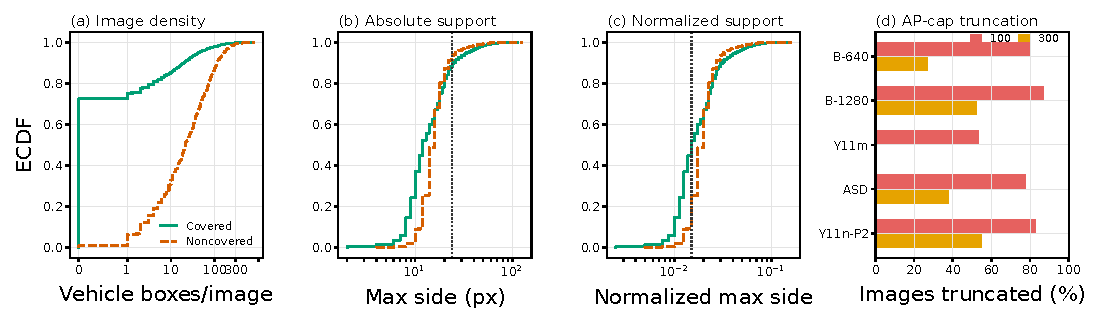
\includegraphics[width=.98\textwidth]{../figures/fig_supplement_coverage_cap.pdf}
\caption{Ancillary qualification records. (a)--(c) AI-TOD covered and noncovered image groups differ in density and support; vertical lines mark 24 px and .015. ECDFs in (b) and (c) use individual vehicle boxes. (d) Fractions of the 548 common VisDrone images whose mapped prediction counts exceed maxDets 100 or 300. At maxDets 2000, all five fractions are zero.}\label{fig:supp-qualification}
\end{figure*}

Figure~\ref{fig:supp-qualification} separates two boundary checks that precede metric interpretation. The AI-TOD density gap is visible at the image level, while the box-level curves show that coverage selection also changes the support composition of the observed target. The cap panel uses mapped vehicle predictions before AP truncation: a low cap would modify the prediction set for every configuration by a different amount. The registered cap of 2,000 exceeds the observed per-image maximum of 1,881 and therefore preserves every mapped prediction.

\begin{figure*}[!t]
\centering
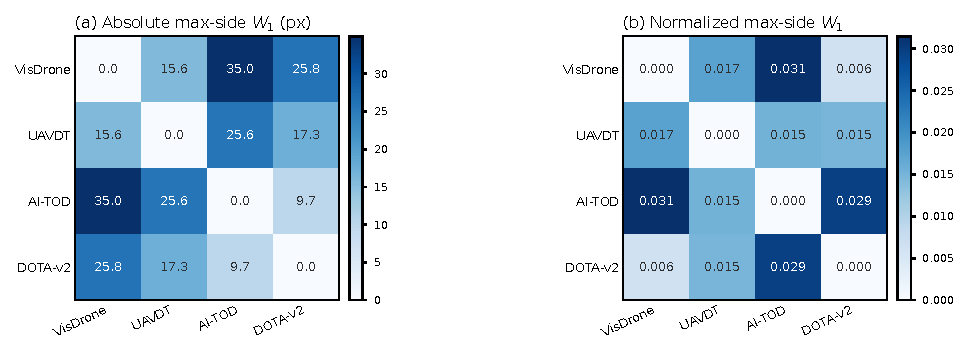
\includegraphics[width=.86\textwidth]{../figures/fig_supplement_structural_distance.pdf}
\caption{Pairwise empirical Wasserstein distances for full-annotation vehicle support. (a) Absolute max side is scale covariant. (b) Normalized max side is resize invariant but retains nonzero source distances. DOTA-v2 is structural-only evidence and does not enter prediction-conditioned metric or rank claims.}\label{fig:supp-distance}
\end{figure*}

Figure~\ref{fig:supp-distance} provides the structural context omitted from the main figures. Normalization changes the coordinate system and greatly compresses the numerical scale, but it does not collapse the four empirical distributions. In particular, the largest normalized pairwise distance is .031 between VisDrone and AI-TOD, whereas VisDrone and DOTA-v2 differ by .006. These are distributional distances, not annotation-quality scores, and no detector result is inferred from them.

\begin{figure*}[!t]
\centering
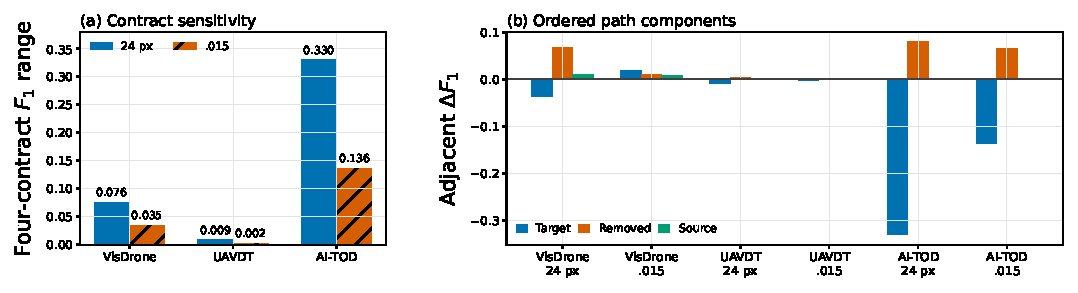
\includegraphics[width=.96\textwidth]{../figures/fig_supplement_contract_summary.pdf}
\caption{Cross-source summary of the registered headline path. (a) Four-contract micro-$F_1$ ranges. (b) Adjacent path changes, preserving the registered order rather than treating them as order-free causal components. Normalized .015 reduces the range in all three sources but leaves source-dependent residual sensitivity.}\label{fig:supp-contract}
\end{figure*}

\section{Reproducibility Record}
\begin{table}[!t]
\centering
\caption{Minimal replay chain in the released repository.}\label{tab:repro}
\scriptsize
\setlength{\tabcolsep}{2.0pt}\renewcommand{\arraystretch}{1.03}
\begin{tabular}{p{.22\columnwidth}p{.70\columnwidth}}
\toprule
Audit object & Released record or script\\
\midrule
Coverage gate & \texttt{outputs/coverage\_qualification/} and \texttt{evaluate\_aitod\_coverage\_qualification.py}\\
Support denominator & \texttt{outputs/scale/box\_scale\_records.parquet} and raw-coverage manifests\\
Contract path & \texttt{outputs/contract\_path/}, \texttt{contract\_path.py}, and \texttt{evaluate\_contract\_path\_headlines.py}\\
Metric-qualified rank & \texttt{outputs/metric\_qualified\_rank/} and \texttt{evaluate\_metric\_qualified\_visdrone\_rank.py}\\
Figures and tests & Three \texttt{build\_*.py} scripts; contract, support, matching, and AP regression tests\\
Repository & \url{https://github.com/Marchematics/aerial-evaluation-audit}\\
\bottomrule
\end{tabular}
\end{table}

The data-free release provides configurations, derived records, scripts, and SHA-256 checksums. Licensed imagery, trained weights, and raw prediction caches remain external and are referenced by manifest path and hash. Reproduction order is coverage $\rightarrow$ support $\rightarrow$ contract endpoints/ledger $\rightarrow$ paired metric qualification $\rightarrow$ figures.

\end{document}
